\documentclass{article}

\title{EE 371 Autumn 2016 - Lab 2}
\date{\today}
\author{William Li, Dawn Liang, Jun Park}

% general document formatting
\usepackage[margin=1in]{geometry}
\usepackage[document]{ragged2e}
\usepackage{times}

\usepackage{titlesec}
\titleformat{\section}{\Large\bfseries}{\thesection}{0.5em}{\uppercase}

% formatting for code & floats
\usepackage{listings}
\usepackage{color}
\usepackage{graphicx}
\usepackage{float}
\usepackage{wrapfig}

\definecolor{dkgreen}{rgb}{0,0.6,0}
\definecolor{gray}{rgb}{0.5,0.5,0.5}
\definecolor{mauve}{rgb}{0.58,0,0.82}

\lstset{frame=tb,
  language=Verilog,
  aboveskip=3mm,
  belowskip=3mm,
  showstringspaces=false,
  columns=flexible,
  basicstyle={\small\ttfamily},
  numbers=none,
  numberstyle=\tiny\color{gray},
  keywordstyle=\color{blue},
  commentstyle=\color{dkgreen},
  stringstyle=\color{mauve},
  breaklines=true,
  breakatwhitespace=true,
  tabsize=3
}


% write-up
\begin{document}

\newcommand{\namesigdate}[2][5cm]{
  \begin{tabular}{@{}p{#1}@{}}
    #2 \\[2\normalbaselineskip] \hrule \\[0pt]
    {\small \textit{Signature}} \\[2\normalbaselineskip] \hrule \\[0pt]
    {\small \textit{Date}}
  \end{tabular}
}

\pagenumbering{gobble}
\maketitle
\newpage

\paragraph{signatures} We certify that the work in this report is our own, and that any work that is not ours is cited.
\paragraph{} \noindent \namesigdate{William Li} \hfill \namesigdate{Dawn Liang} \hfill \namesigdate{Jun Park}
\paragraph{contributions} Jun worked on designing the project, drawing diagrams and building state machines, wrote iterations of the modules, and wrote the test part of the write-up. William wrote the C program and the write-up for the C program, wrote the poundOccupied module. Dawn worked on designing the project, wrote the overall module and the final iteration of the other modules, wrote the Requirements \& Design Spec and Functional Decomposition, and compiled and formatted the final write-up.
\newpage

\tableofcontents
\newpage

\pagenumbering{arabic}

\section{Abstract}
\paragraph{} In this lab, we were introduced to our first digital design project. We designed and built a simple time-dependent system, a poundlock control system. We wrote requirement and design specifications as well as a functional decomposition for the VHDL program, to help us organise the design process. We then wrote our modules in Verilog and tested our design in simulation using iverilog and gtkwave as well as in hardware on the Altera DE1-SoC board. Additionally, we furthered our knowledge of the C language by writing a C program using pointers. These projects helped us develop our skills in designing hardware and software programs.


\section{Introduction}
\paragraph{} The first part of the lab focuses on building systems in VHDL (Verilog Hardware Description Language). We decomposed the system at a high level in terms of requirements, design, and functions, and wrote specifications for each. This helped us decide the components of our design. We built and tested each submodule in simulation using iverilog and gtkwave, and later integrated them together and simulated them again. Finally, we downloaded the system via Quartus to the DE1-SoC board and checked its behaviour in hardware. We used Signal Tap II Logic Analyser to debug our system and verify proper functionality. In the second part of the lab, we wrote a simple C program using pointer references, to introduce and familiarise ourselves with the concepts.


\section{Discussion}
	\subsection{Design}
		\subsubsection{Design Specification - VHDL}
  		\paragraph{Abstract} At various points along the canal system of Venice, gondolas must move between areas of significantly differing water levels. In order to do so smoothly, pound locks are in place to facilitate both transportation of gondolas and maintenance of water levels. These locks are controlled by a digital system we have designed and built.

      \paragraph{Introduction} The system for controlling locks will allow gondolas to pass between areas of the canal of uneven water levels. Upon arrival, the gondola must signal the lock to initiate the process, enter the lock, wait as it is raised/lowered, and then exit the lock to continue its journey. The opening/closing of gates and raising/lowering of water levels are controlled by a lock operator.

      \paragraph{Inputs to the system}
      \paragraph{} User Inputs
      \begin{itemize}
        \item fiveMinsTillArrival: signal from the gondola that it will be arriving in at least five minutes, to prompt the lock to adjust water levels and open the gates (1-bit trigger true/false)
        \begin{itemize}
          \item SA0: the lock will not know when there is a boat arriving, so it will never prepare the arrival gates for entry.
          \item SA1: the lock will behave as if there is always another boat in the queue. It will function as normal, except that after each boat exits, the lock will immediately prepare itself for another boat to enter.
        \end{itemize}

        \item incrWaterLevel: control signal to increase the water level inside the lock, to bring the water levels inside and outside the lock close enough that the gates can open (1-bit trigger true/false)
        \begin{itemize}
          \item SA0: the lock will never fill the lock up to the higher outside water level
          \item SA1: the lock will be constantly filled to the higher outside water level
        \end{itemize}

        \item decrWaterLevel: control signal to decrease the water level inside the lock, to bring the water levels inside and outside the lock close enough that the gates can open (1-bit trigger true/false)
        \begin{itemize}
          \item SA0: the lock will never drain the lock down to the lower outside water level
          \item SA1: the lock will be constantly drain to the lower outside water level
        \end{itemize}

        \item reset: empties the lock to the lower outside water level, lets the boats out, and seals the gates (1-bit switch true/false)
        \begin{itemize}
          \item SA0: the lock will not be able to reset, but otherwise function as normal
          \item SA1: the lock will be constantly in the reset state (no boat, drained, gates sealed)
        \end{itemize}
      \end{itemize}

      \paragraph{} Environmental controls
      \begin{itemize}
        \item arrivOutsideLevel: the water level outside the lock, on the arrival side, determining whether the arrival gate can open (4-bit binary 0-15, each unit corresponds to 0.3125ft)
        \item deptOutsideLevel: the water level outside the lock, on the departure side, determining whether the departure gate can open (4-bit binary 0-15, each unit corresponds to 0.3125ft)
        \begin{itemize}
          \item If any of the bits fault for either signal, the range of possible values is restricted to those attainable with the stuck bit
        \end{itemize}
      \end{itemize}

      \paragraph{} Internal signals
      \begin{itemize}
        \item poundOccupied: whether there is currently a gondola in the lock, since if the lock is occupied, the next boat cannot enter (1-bit true/false)
        \begin{itemize}
          \item SA0: the lock will always act as if there is not a boat in the lock, 
          \item SA1: the lock will always act as if there is a boat in the lock, so it will not open the arrival gates to let boats enter
        \end{itemize}

        \item insideWaterLevel: the water level inside the lock, determining whether the gates can open (4-bit binary 0-15, each unit corresponds to 0.3125ft)
        \begin{itemize}
          \item If any of the bits fault, the range of possible values is restricted to those attainable with the stuck bit
        \end{itemize}

        \item arrivGateOpen: whether the door on the arrival side is open (1-bit true/false)
        \item deptGateOpen: whether the door on the departure side is open (1-bit true/false)
        \begin{itemize}
          \item SA0: If either gate is sealed, boats cannot enter/exit the lock
          \item SA1: If either gate is open, the lock cannot adjust its inside water level
        \end{itemize}
      \end{itemize}

      \paragraph{Outputs of major functions}
      \begin{itemize}
        \item gateOpenClose: opens/closes the lock gates, allowing gondolas to enter/exit the lock (1-bit open/closed gate)
        \begin{itemize}
          \item SA0: the gates are constantly closed, not allowing any boats through the lock
          \item SA1: the gates are constantly open, unable to adjust the water level inside the lock and thus not allowing any boats through
        \end{itemize}

        \item incrWaterLevel: increases the water level inside the lock, matching it to the outside higher water level so that the gate can open (4-bit binary 0-15, each unit corresponds to 0.3125ft change in the inside water level)
        \item decrWaterLevel: decreases the water level inside the lock, matching it to the outside higher water level so that the gate can open (4-bit binary 0-15, each unit corresponds to 0.3125ft change in the inside water level)
          \begin{itemize}
            \item The lock can adjust its water level by up to 5ft (each bit corresponds to 0.3125 ft)
            \item The lock takes up to 7 minutes to drain, 8 minutes to fill (each clock edge corresponds to 30s)
            \item If any of the bits fault, the range of possible values is restricted to those attainable with the stuck bit, so the lock potentially cannot fill/drain sufficiently to open the gates
          \end{itemize}
      \end{itemize}

    \subsubsection{Design Specification - C Program}
      \paragraph{Abstract} The project2.c program is a project that teaches us the fundamentals of pointers and references in the C programming language. Written in C and in the CodeBlocks IDE, our program contained hard coded values which are then processed into a simple equation. The result is then outputted to the user. Our program results matched our expectations, outputting the correct answer every time.

      \paragraph{Introduction} This project gave us a continuation to our C programming knowledge and experience working in the CodeBlocks IDE. The result of this project was a program that calculates the answer of the equation from a few hardcoded values (as described in the specifications) and outputs the value to the user.

      \paragraph{Inputs to the system} There were no inputs into this program.
      \paragraph{Outputs of major functions} The output value of the program is an integer value, which in this case is always 5.

      \paragraph{Major functions} The project2.c program calculates the solution to the expression $((A + B) \times (C - D)) / E$, where A, B, C, D, and E are hardcoded to be 22, 17, 6, 4 and 9 respectively.

    \subsubsection{Design Procedure}
  		\paragraph{VHDL Design} The basic functionality of the lock was decomposed into an overall central module, opening/closing the gates, and adjusting the water level inside the lock. Each binary unit for water levels corresponds to 0.3125ft, for modeling water level heights; each clock cycle corresponds to half a minute, for modeling timing.

      \paragraph{} Functional Decomposition
      \begin{itemize}
        \item Monitoring overall variables for the lock, like its state \& external interactions
        \begin{itemize}
          \item locations of boats
          \item interactions with boats
          \item reset
        \end{itemize}

        \item Open/close gates: the gates open/close to let boats enter/exit the lock
        \begin{itemize}
          \item Input gate-opening conditions must be met (boat incoming/departing, comparing the water level inside the gate to the water level outside the gate, lock empty in the case of the arrival gate)
          \item the gates are not FSMs, since their output does not depend on their present state; implemented using combinational logic
        \end{itemize}

        \item Adjust water levels: the lock fills/drains to match inside and outside water levels, so that the gates can open
        \begin{itemize}
          \item Keeping track of and updating the inside water level for draining/filling the lock
          \item Filling/draining is bounded by the external water levels
          \item Input fill/drain conditions must be met (gates closed, receive signal)
          \item Water level matches counter behaviour very closely, so we used an enable-counter that counts up/down to min/max values based on inputs
        \end{itemize}
      \end{itemize}

      % functional flowchart
      \begin{figure}[H]
        \centering
        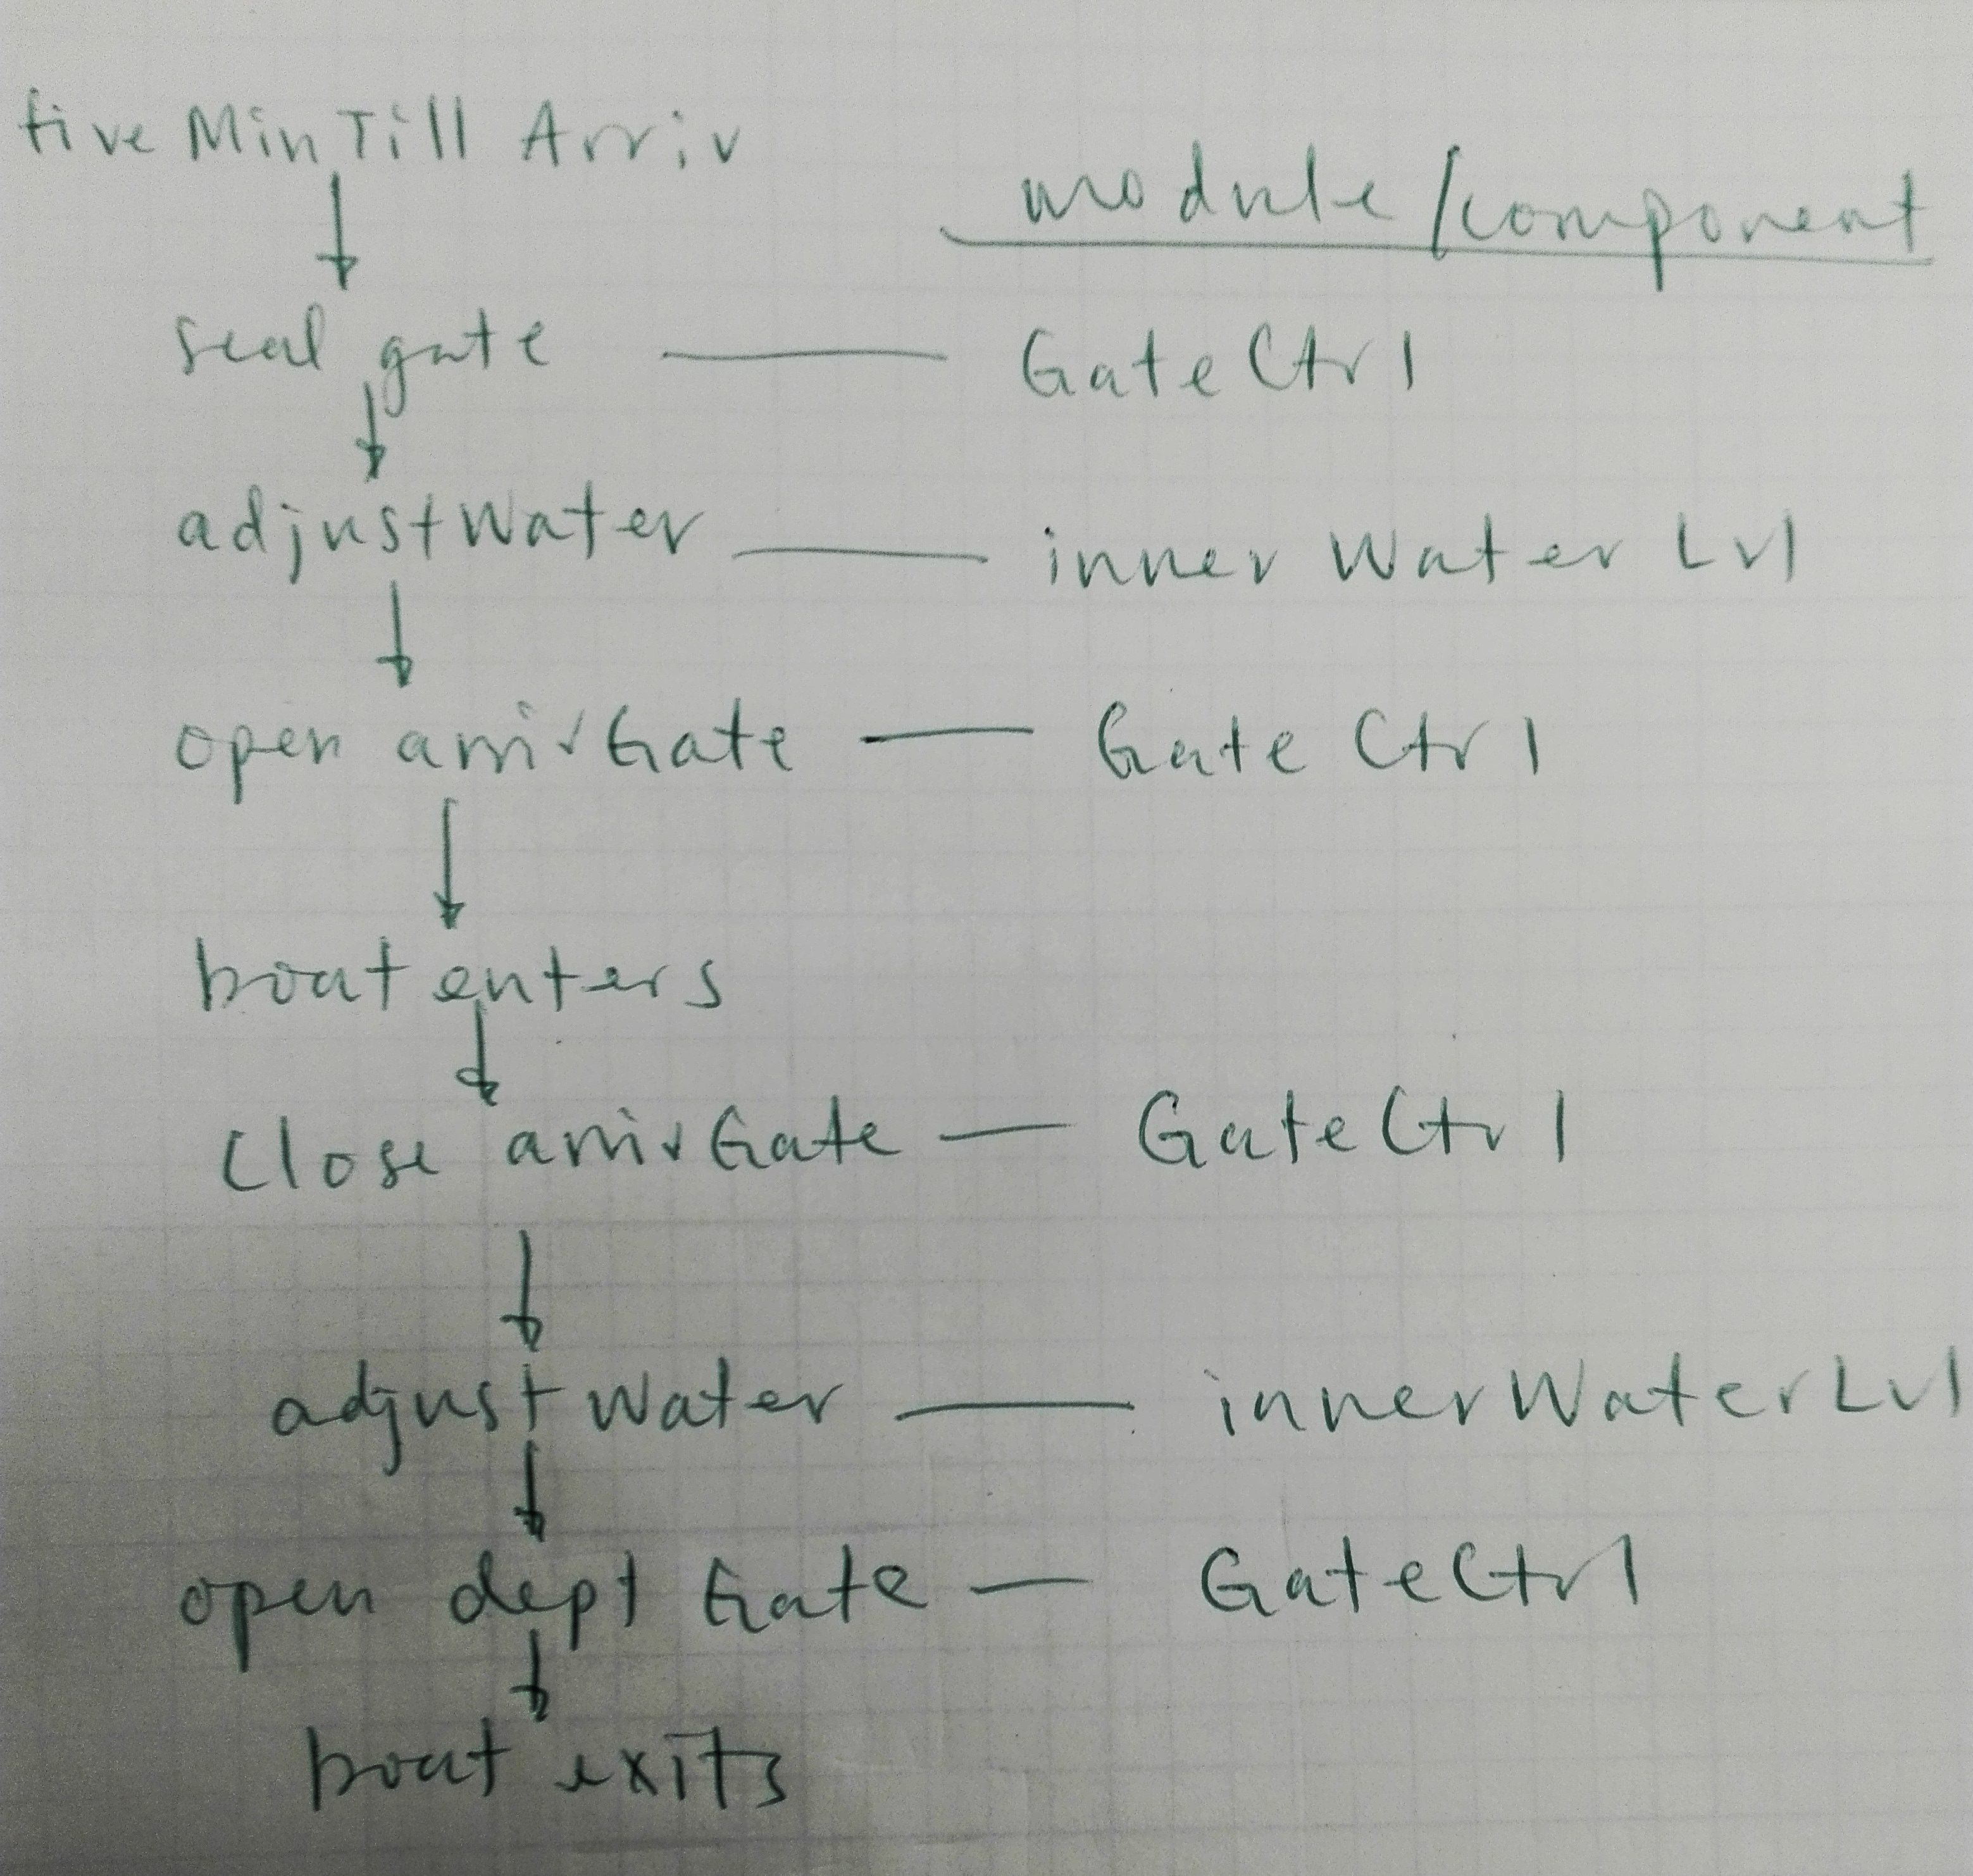
\includegraphics[width=0.75\linewidth]{figures/functional_flowchart.jpeg}
        \caption{Functional flowchart}
        \label{fig:functional_flowchart}
      \end{figure}

      % functional block diagram{}
      \begin{figure}[H]
        \centering
        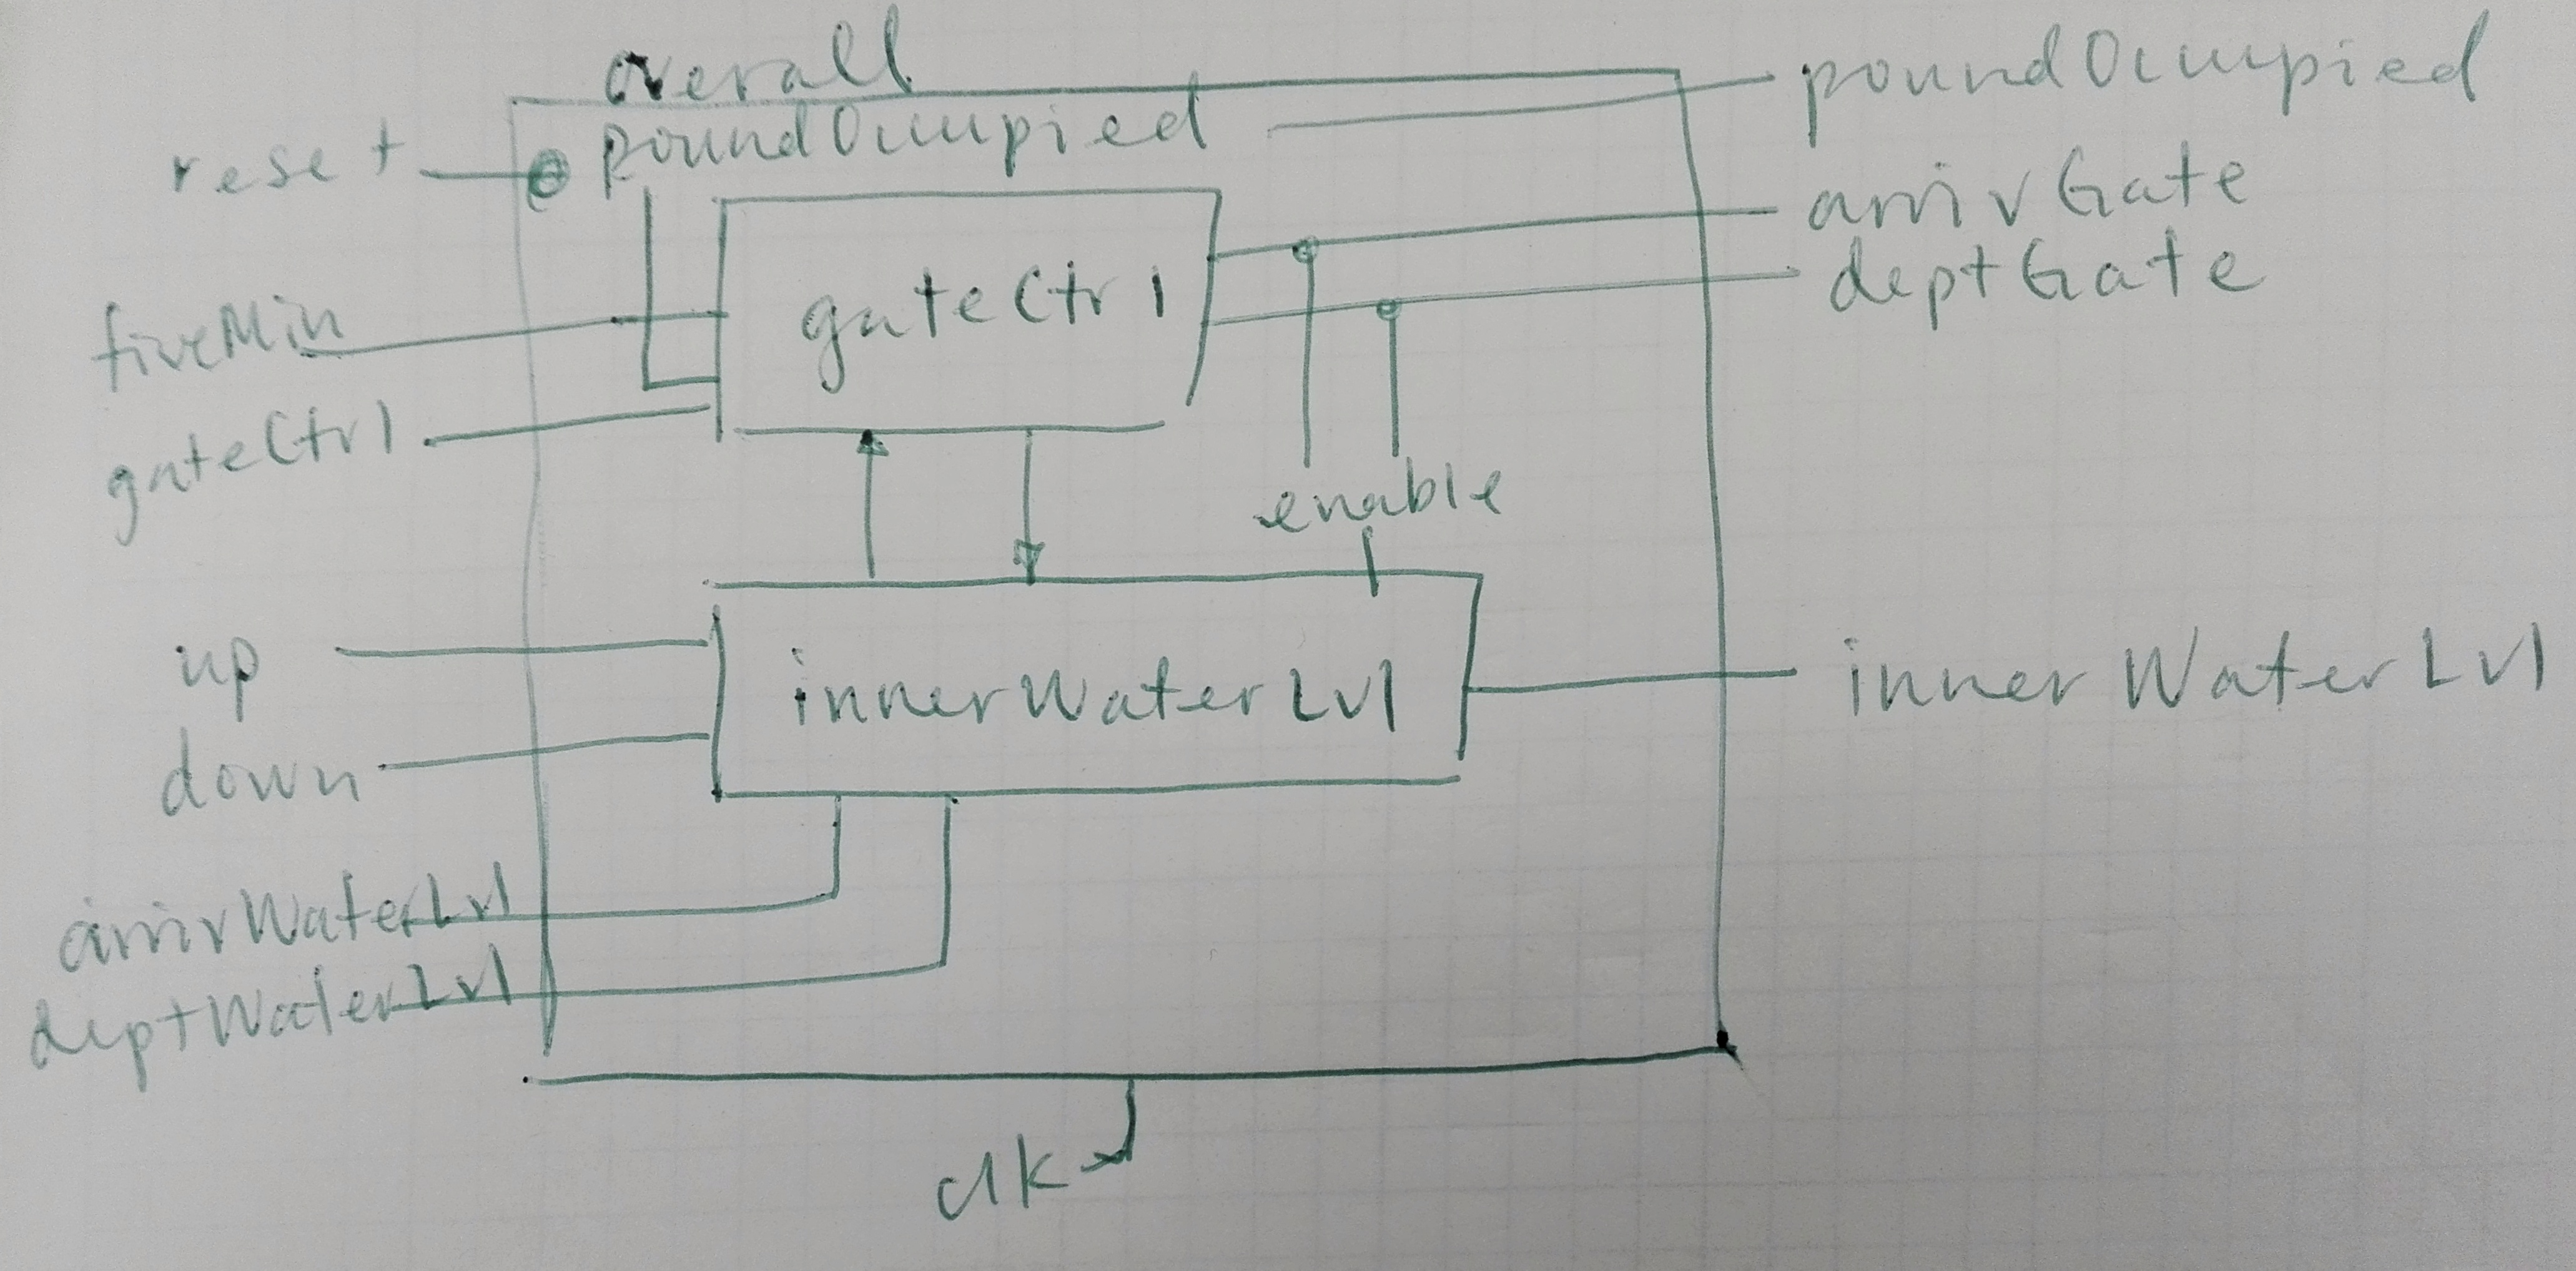
\includegraphics[width=0.75\linewidth]{figures/functional_blockdiagram.jpeg}
        \caption{Functional block diagram}
        \label{fig:functional_blockdiagram}
      \end{figure}

      \paragraph{C Program} The C program was designed as a single unit with no additional methods. Since we were required to have very specific inputs into our program, these values were hardcoded into each of the respective variables (A = 22, B = 17, C = 6, D = 4, E = 9). We then made pointers (X1 to X5), and assigned them to each of the variables respectively. From there, we used the pointers in our calculations.

		\subsubsection{System Description}
      \paragraph{VHDL Design} Our system had three major components: an overall system management module, an innerWaterLvl module, and combinational logic for controlling the gates.

      \paragraph{} The overall module managed inputs/outputs to the system and clock division, connected submodules, and used a finite state machine to track the status of the lock.
      \begin{itemize}
        \item Inputs: fiveMinTillArrival, arrivOutsideLvl, deptOutsideLvl, incr, decr, gateCtrl, clock, reset
        \item Outputs: insideWaterLvl, arrivGate, deptGate, poundOccupied
      \end{itemize}
      The overall module handled inverting key inputs (1 for pressed, 0 for unpressed), clock division, an FSM for monitoring the state of the lock (occupied/unoccupied), and connecting up all the submodules. The overall module had to determine which water level was higher in order to connect inputs to the innerWaterLvl module. When reset, the insideWaterLvl becomes 0 and the lock becomes unoccupied.

      \paragraph{} The innerWaterLvl module modeled the water level inside the lock using a counter that counts up/down to a min/max based on inputs, and pauses when disabled
      \begin{itemize}
        \item Inputs: enable, min, max, incr, decr, clock, reset
        \item Outputs: insideWaterLvl
      \end{itemize}
      The counter is told whether to count up/down, and counts up to a max value/down to a min value. It pauses when disabled (enable = 0), and resets to 0. The incr/decr signals must be held down in order to change the water level, and held across a clock edge. Since the water levels vary between 0 and 15bits (0 \& 5ft) and the lock fills/drains at 1bit/clockedge (0.3125ft/30s), the lock takes up to 7 minutes to drain/fill.

      \paragraph{} The gates were implemented using combinatorial logic
      \begin{itemize}
        \item Inputs: fiveMinTillArrival, arrivOutsideLvl, deptOutsideLvl, insideWaterLvl, poundOccupied
        \item Outputs: arrivGate/deptGate (whether the gate is open/closed)
      \end{itemize}
      The arrival and departure gates both open only when the difference between the relevant outer and inner water levels are within 0.3ft of each other. The departure gate opens when prompted, the arrival gate must also have a fiveMinTillArrival signal and the lock must be unoccupied. The gates must be held open for at least two clock edges in order for the boat to enter/exit the lock, and if the lock is occupied, the arrival gate wil not open.

      % C diagram
      \begin{figure}[H]
        \centering
        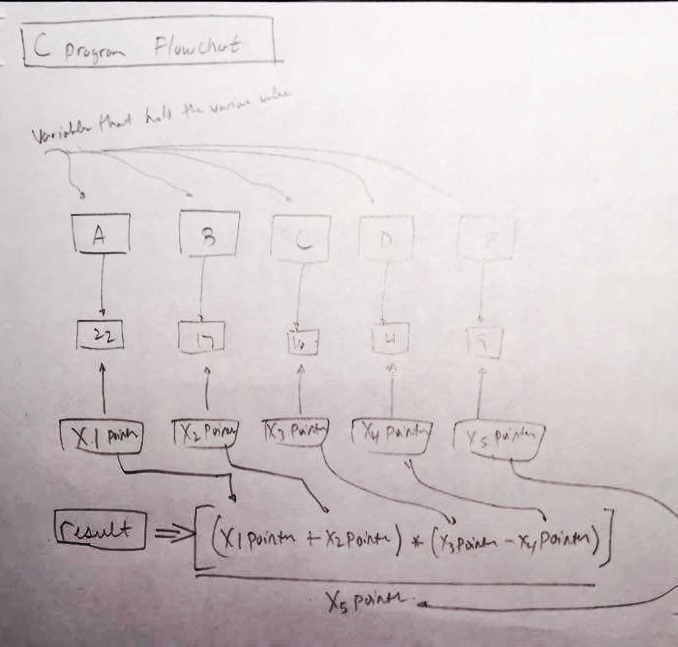
\includegraphics[width=0.75\linewidth]{figures/c/C_diagram.jpeg}
        \caption{C program design specification}
        \label{fig:C_program_design}
      \end{figure}

		\subsubsection{Software Implementation}
      % C flowchart
      \begin{figure}[H]
        \centering
        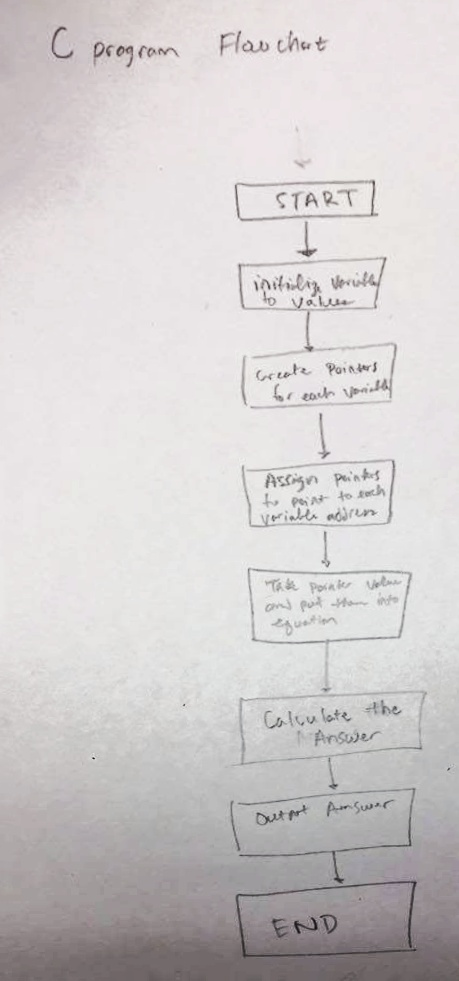
\includegraphics[width=0.6\linewidth]{figures/c/C_flowchart.jpeg}
        \caption{C program information flowchart}
        \label{fig:C_program_flowchart}
      \end{figure}
    
      \paragraph{} The project2.c program was written in C. In the program, we created only one method (the main), where we declared six variables (A, B, C, D, E, result), and initialized each variable to its respective hardcoded value (‘A’ = 22, ‘B’ = 17, ‘C’ = 6, ‘D’ = 4, ‘E’ = 9). The last variable, ‘result’, gets overwritten with the result of the calculations. We then created five pointer variables (labeled X1 to X5) and made each pointer point to the addresses of each variables (X1 $\rightarrow$ A, X2 $\rightarrow$ B, \ldots X5 $\rightarrow$ E).  We then plug the values that are referenced by the pointers into the equation: \[\frac{((A - B) \times (C + D))}{E}\]
      The answer to the equation is then written into the result variable and outputted to the user. Since the program has no inputs, the outputted value is always 5.  

		\subsubsection{Hardware Implementation}
      \paragraph{} Our system was divided into three main functions: a top-level overall system management module, gate control, and adjusting the inner water levels. The overall system handled inputs/outputs and clock timing, kept track of the state of the lock, and connected submodules. To keep track of the state of the lock (poundOccupied signal), the overall module used a finite state machine. Information about the insideWaterLvl and state of the gates was passed between the two submodules using connections in the overall top-level module.

      % overall module diagram
      \begin{figure}[H]
        \centering
        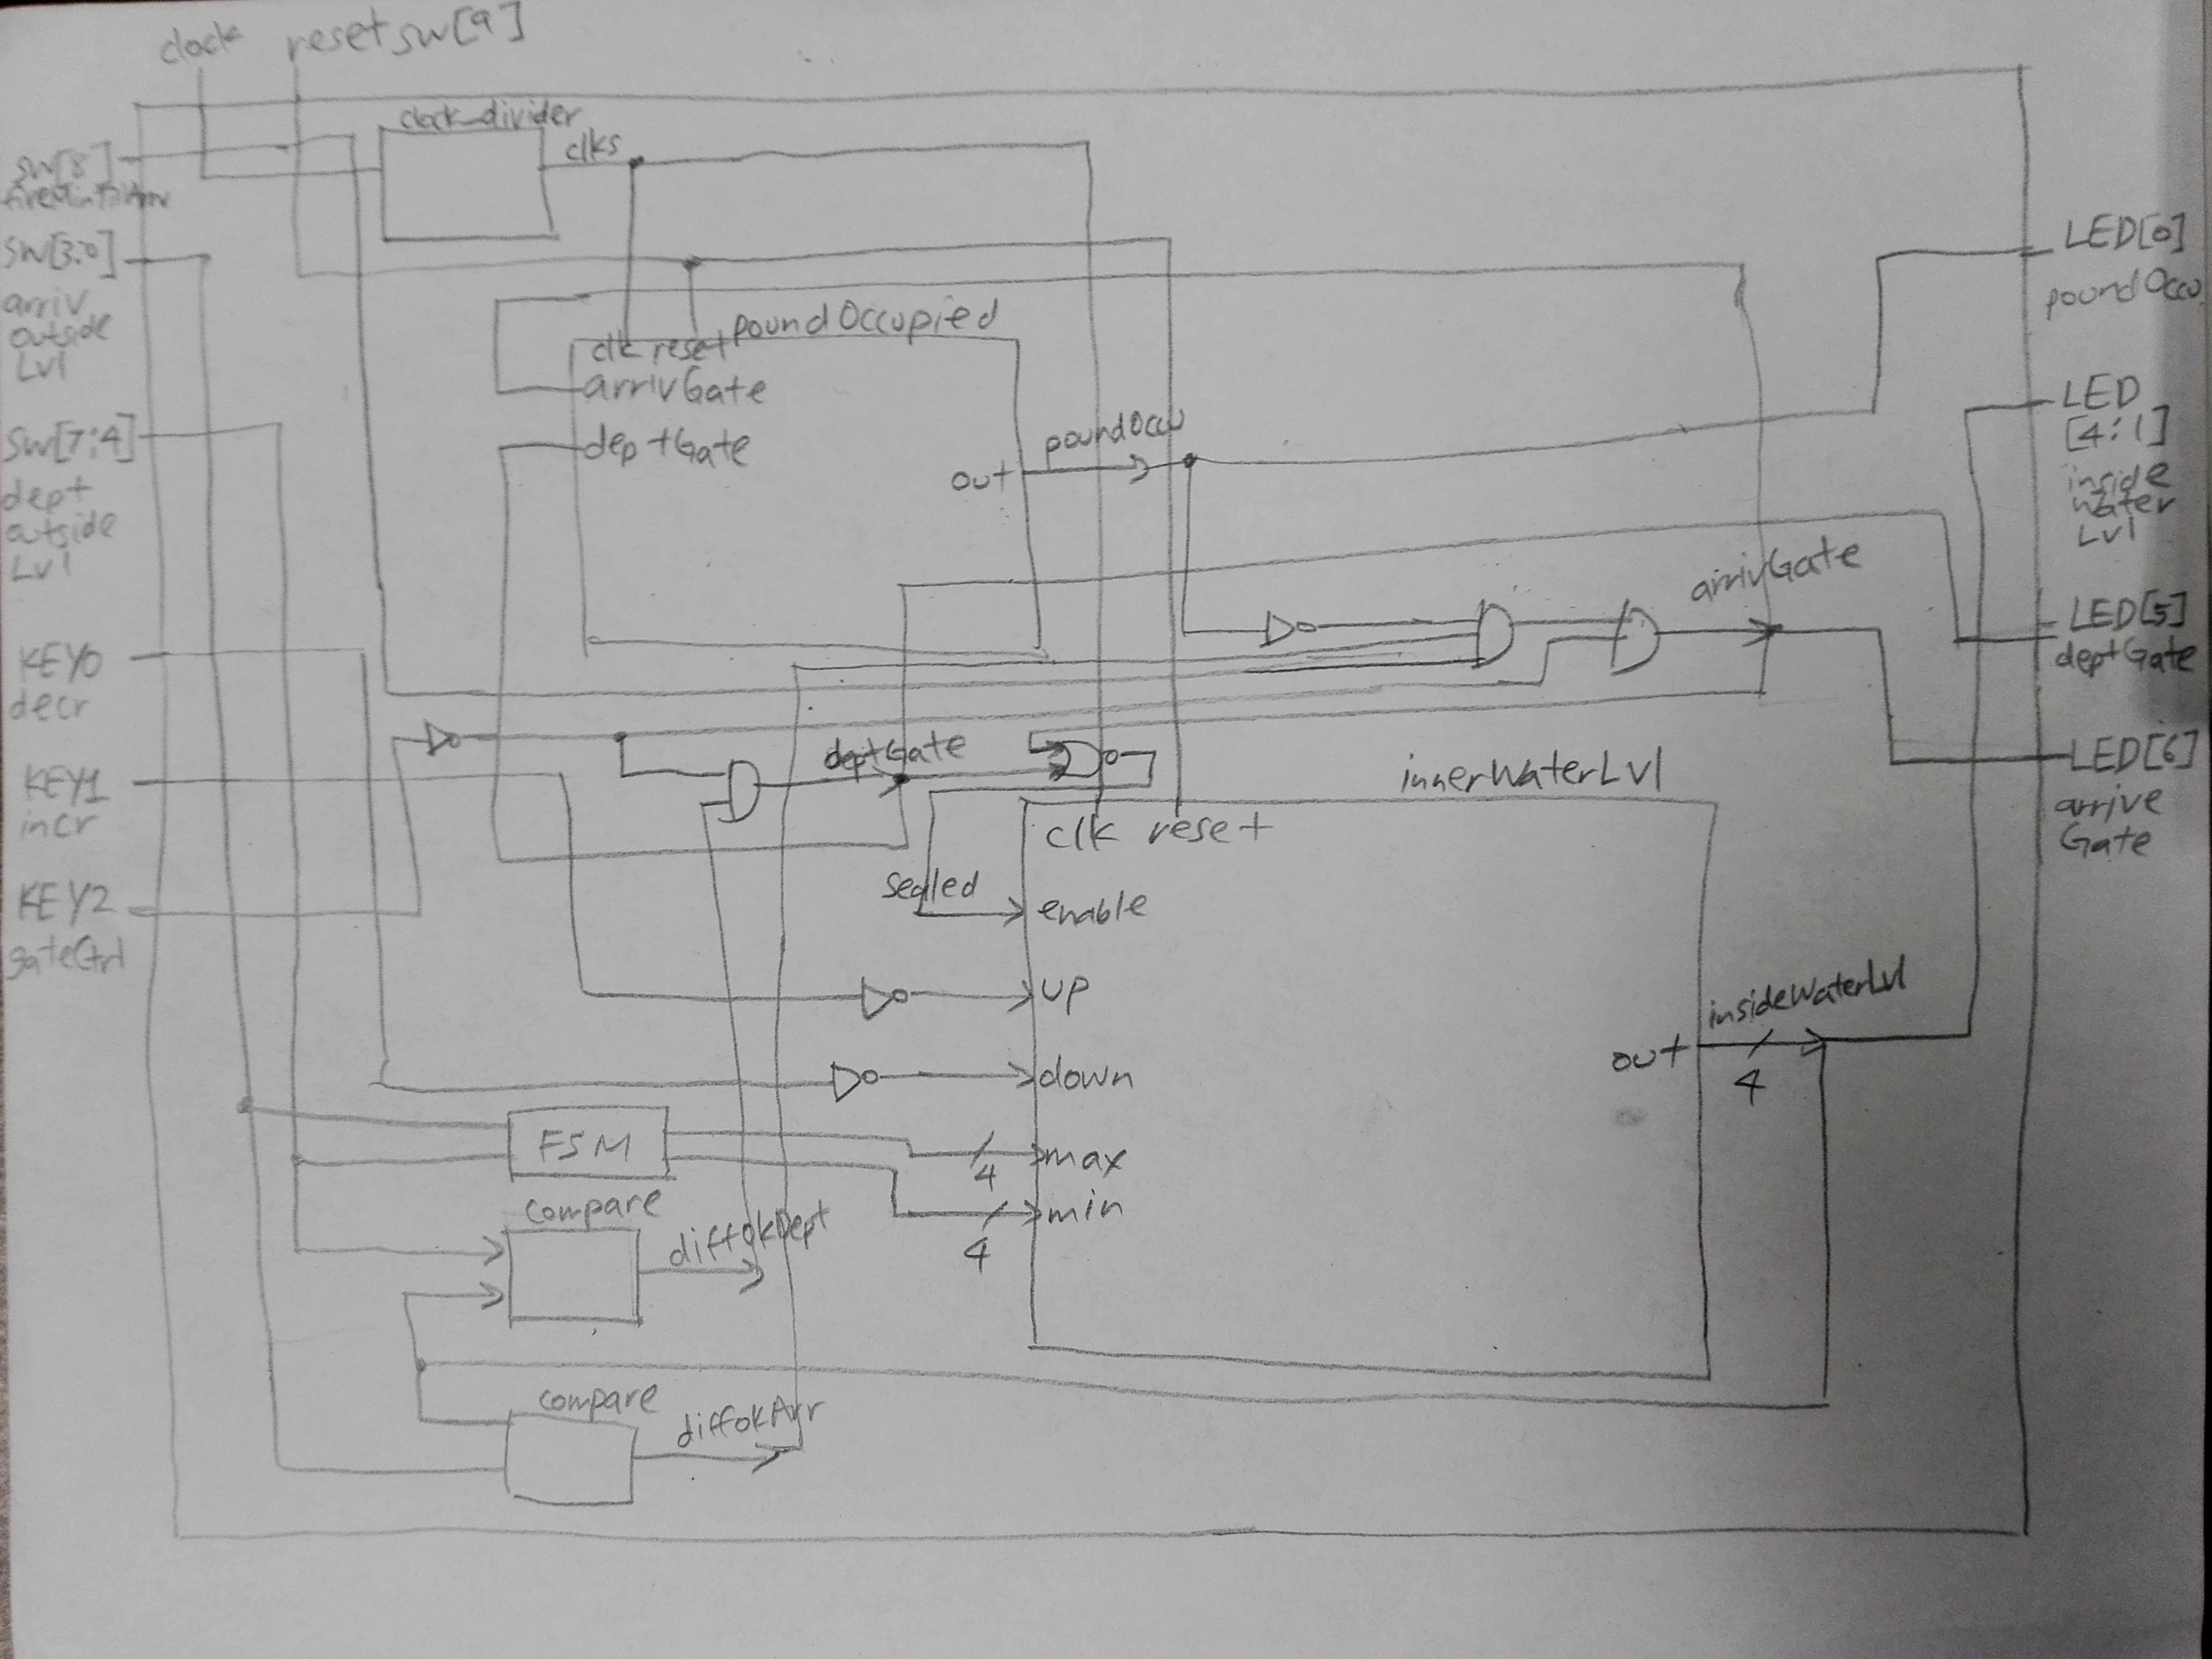
\includegraphics[width=0.75\linewidth]{figures/block_diagrams/overall_diagram.jpeg}
        \caption{Diagram of overall module, including combinational logic for gate control}
        \label{fig:overall_diagram}
      \end{figure}

      % poundOccupied FSM diagram
      \begin{figure}[H]
        \centering
        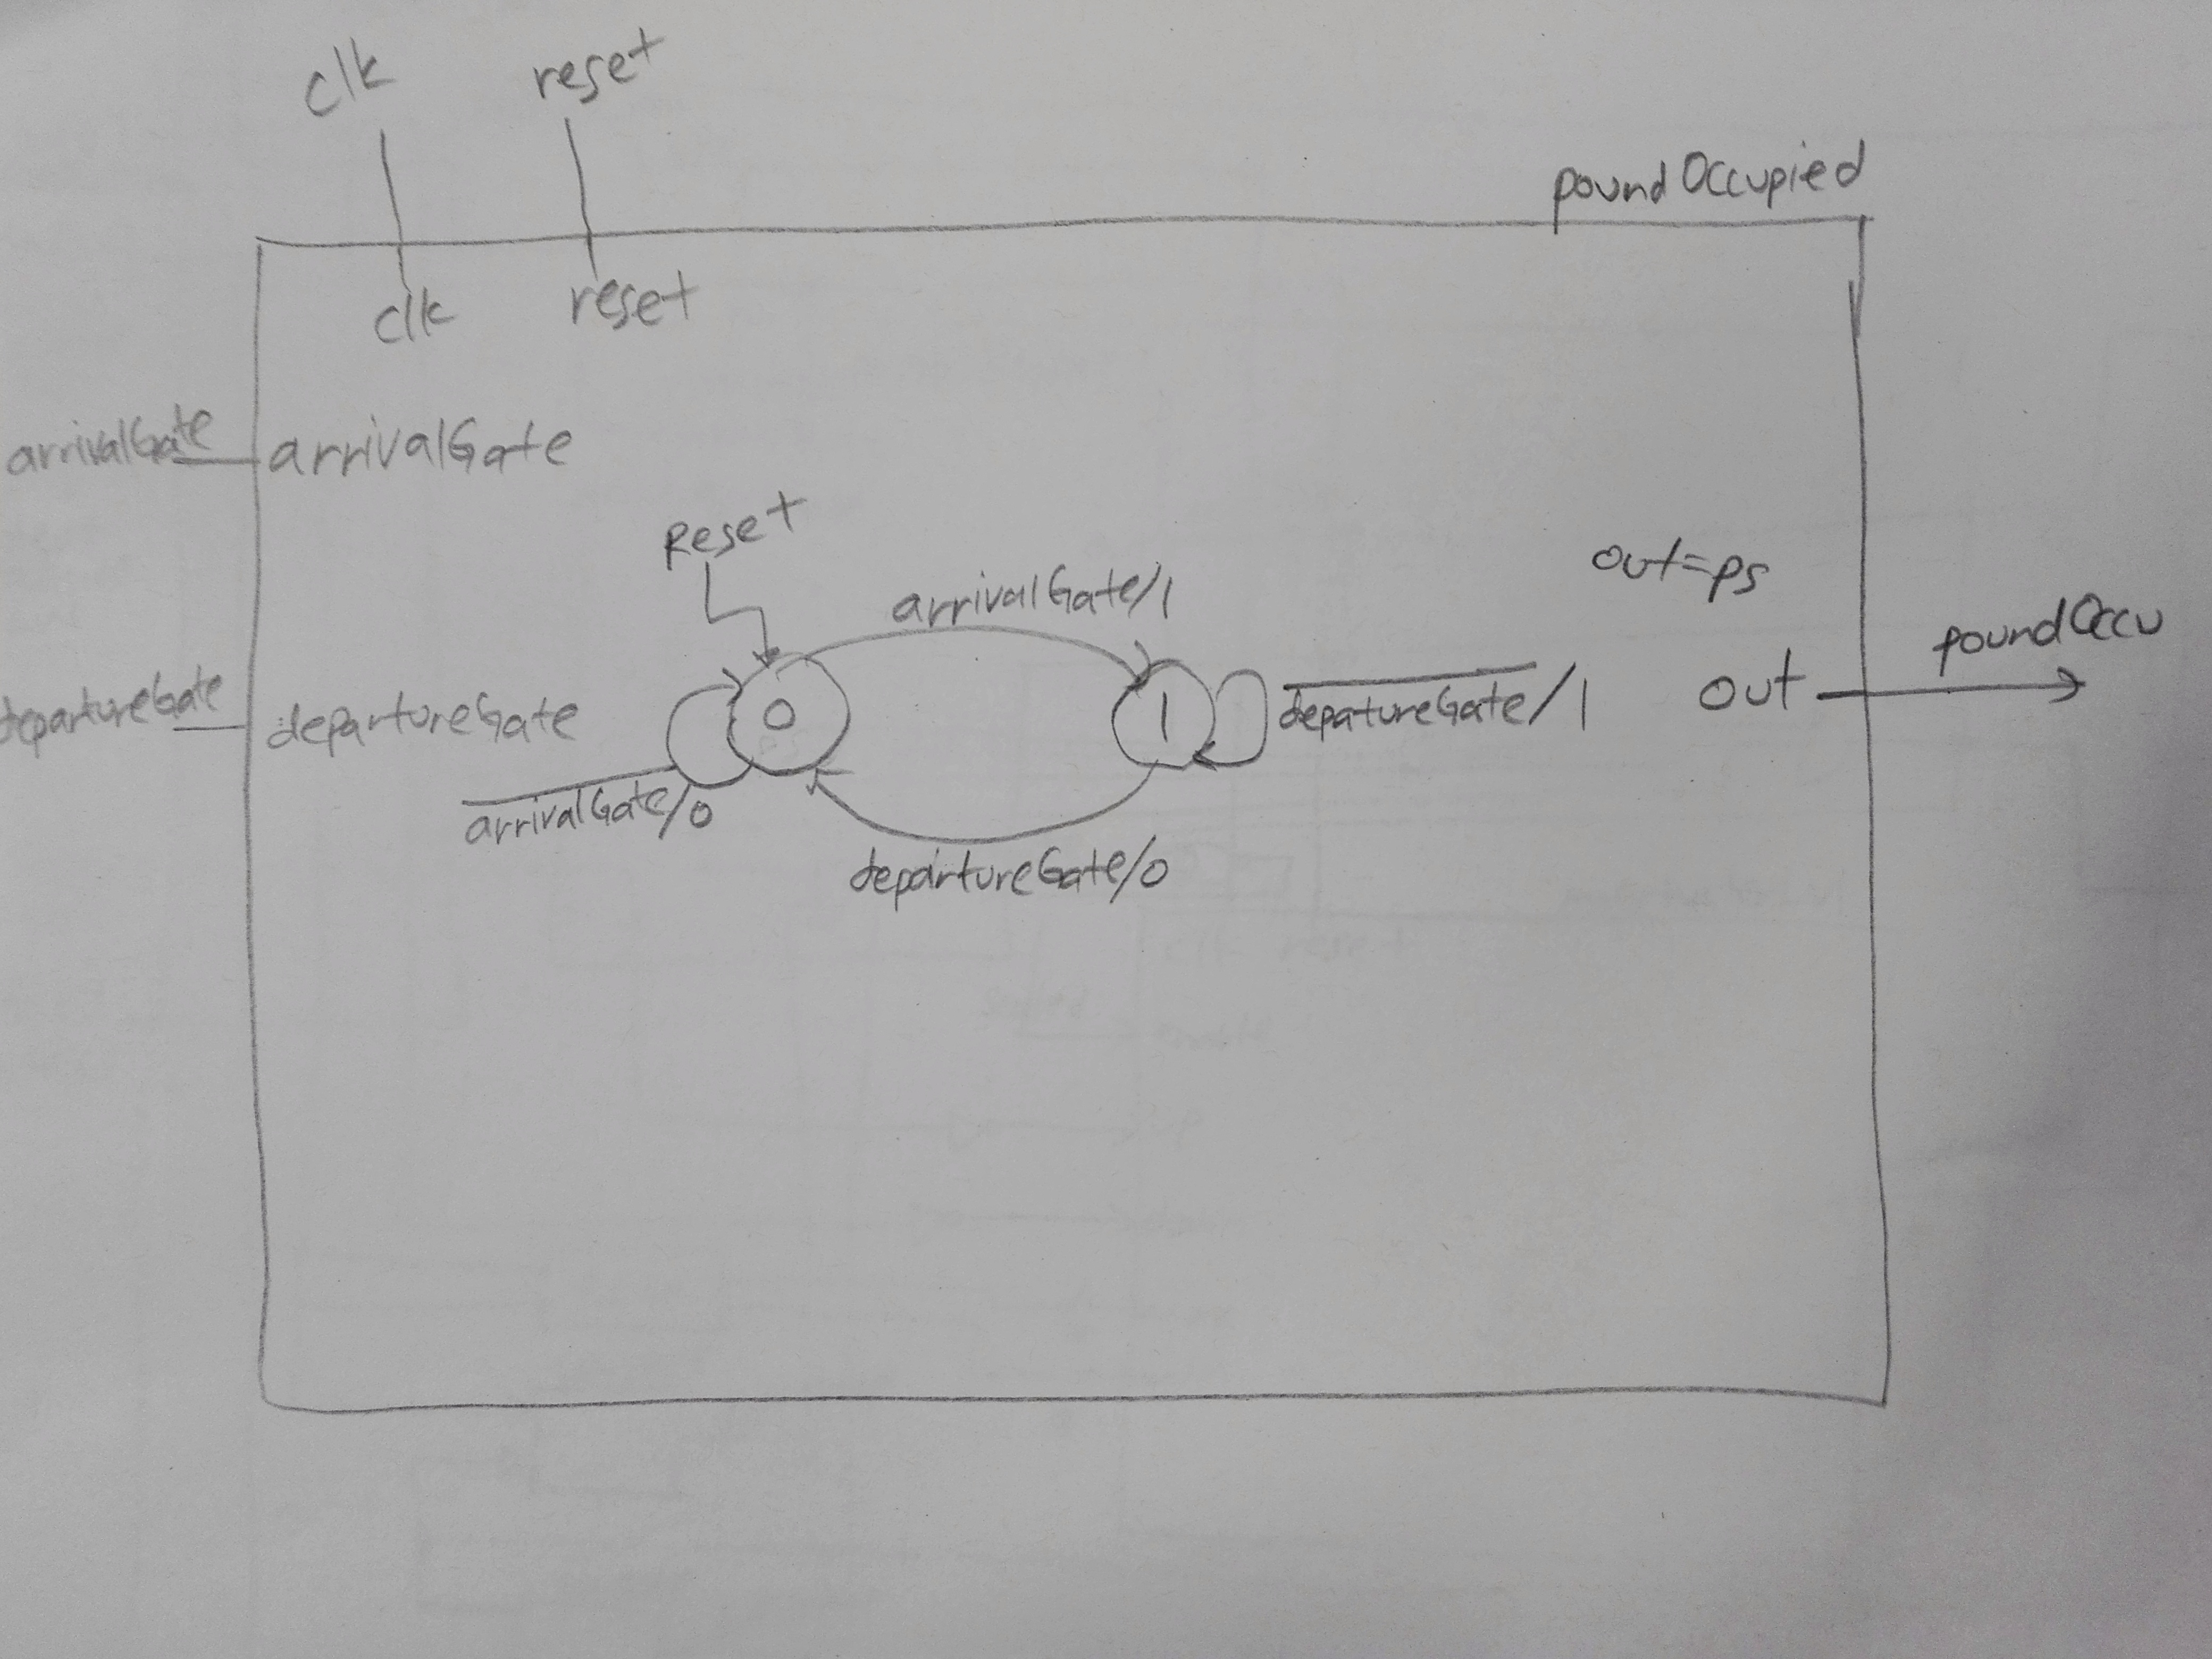
\includegraphics[width=0.75\linewidth]{figures/block_diagrams/poundOccupied_diagram.jpeg}
        \caption{Diagram of poundOccupied FSM module}
        \label{fig:poundOccupied_diagram}
      \end{figure}

      \paragraph{} The innerWaterLvl module controlled the water level inside the lock. It was a generic counter that took min/max values and three control signals (enable, up, down) as input, and gave the counter value as output. The overall module handled the control logic, namely:
      \begin{itemize}
        \item \lstinline{Enable = ~(arrivGate || deptGate)} (if a gate is open, don’t change the water level)
        \item min/max: determining which outside water level was the higher water level, regardless of direction
      \end{itemize}

      % innerWaterLvl module diagram
      \begin{figure}[H]
        \centering
        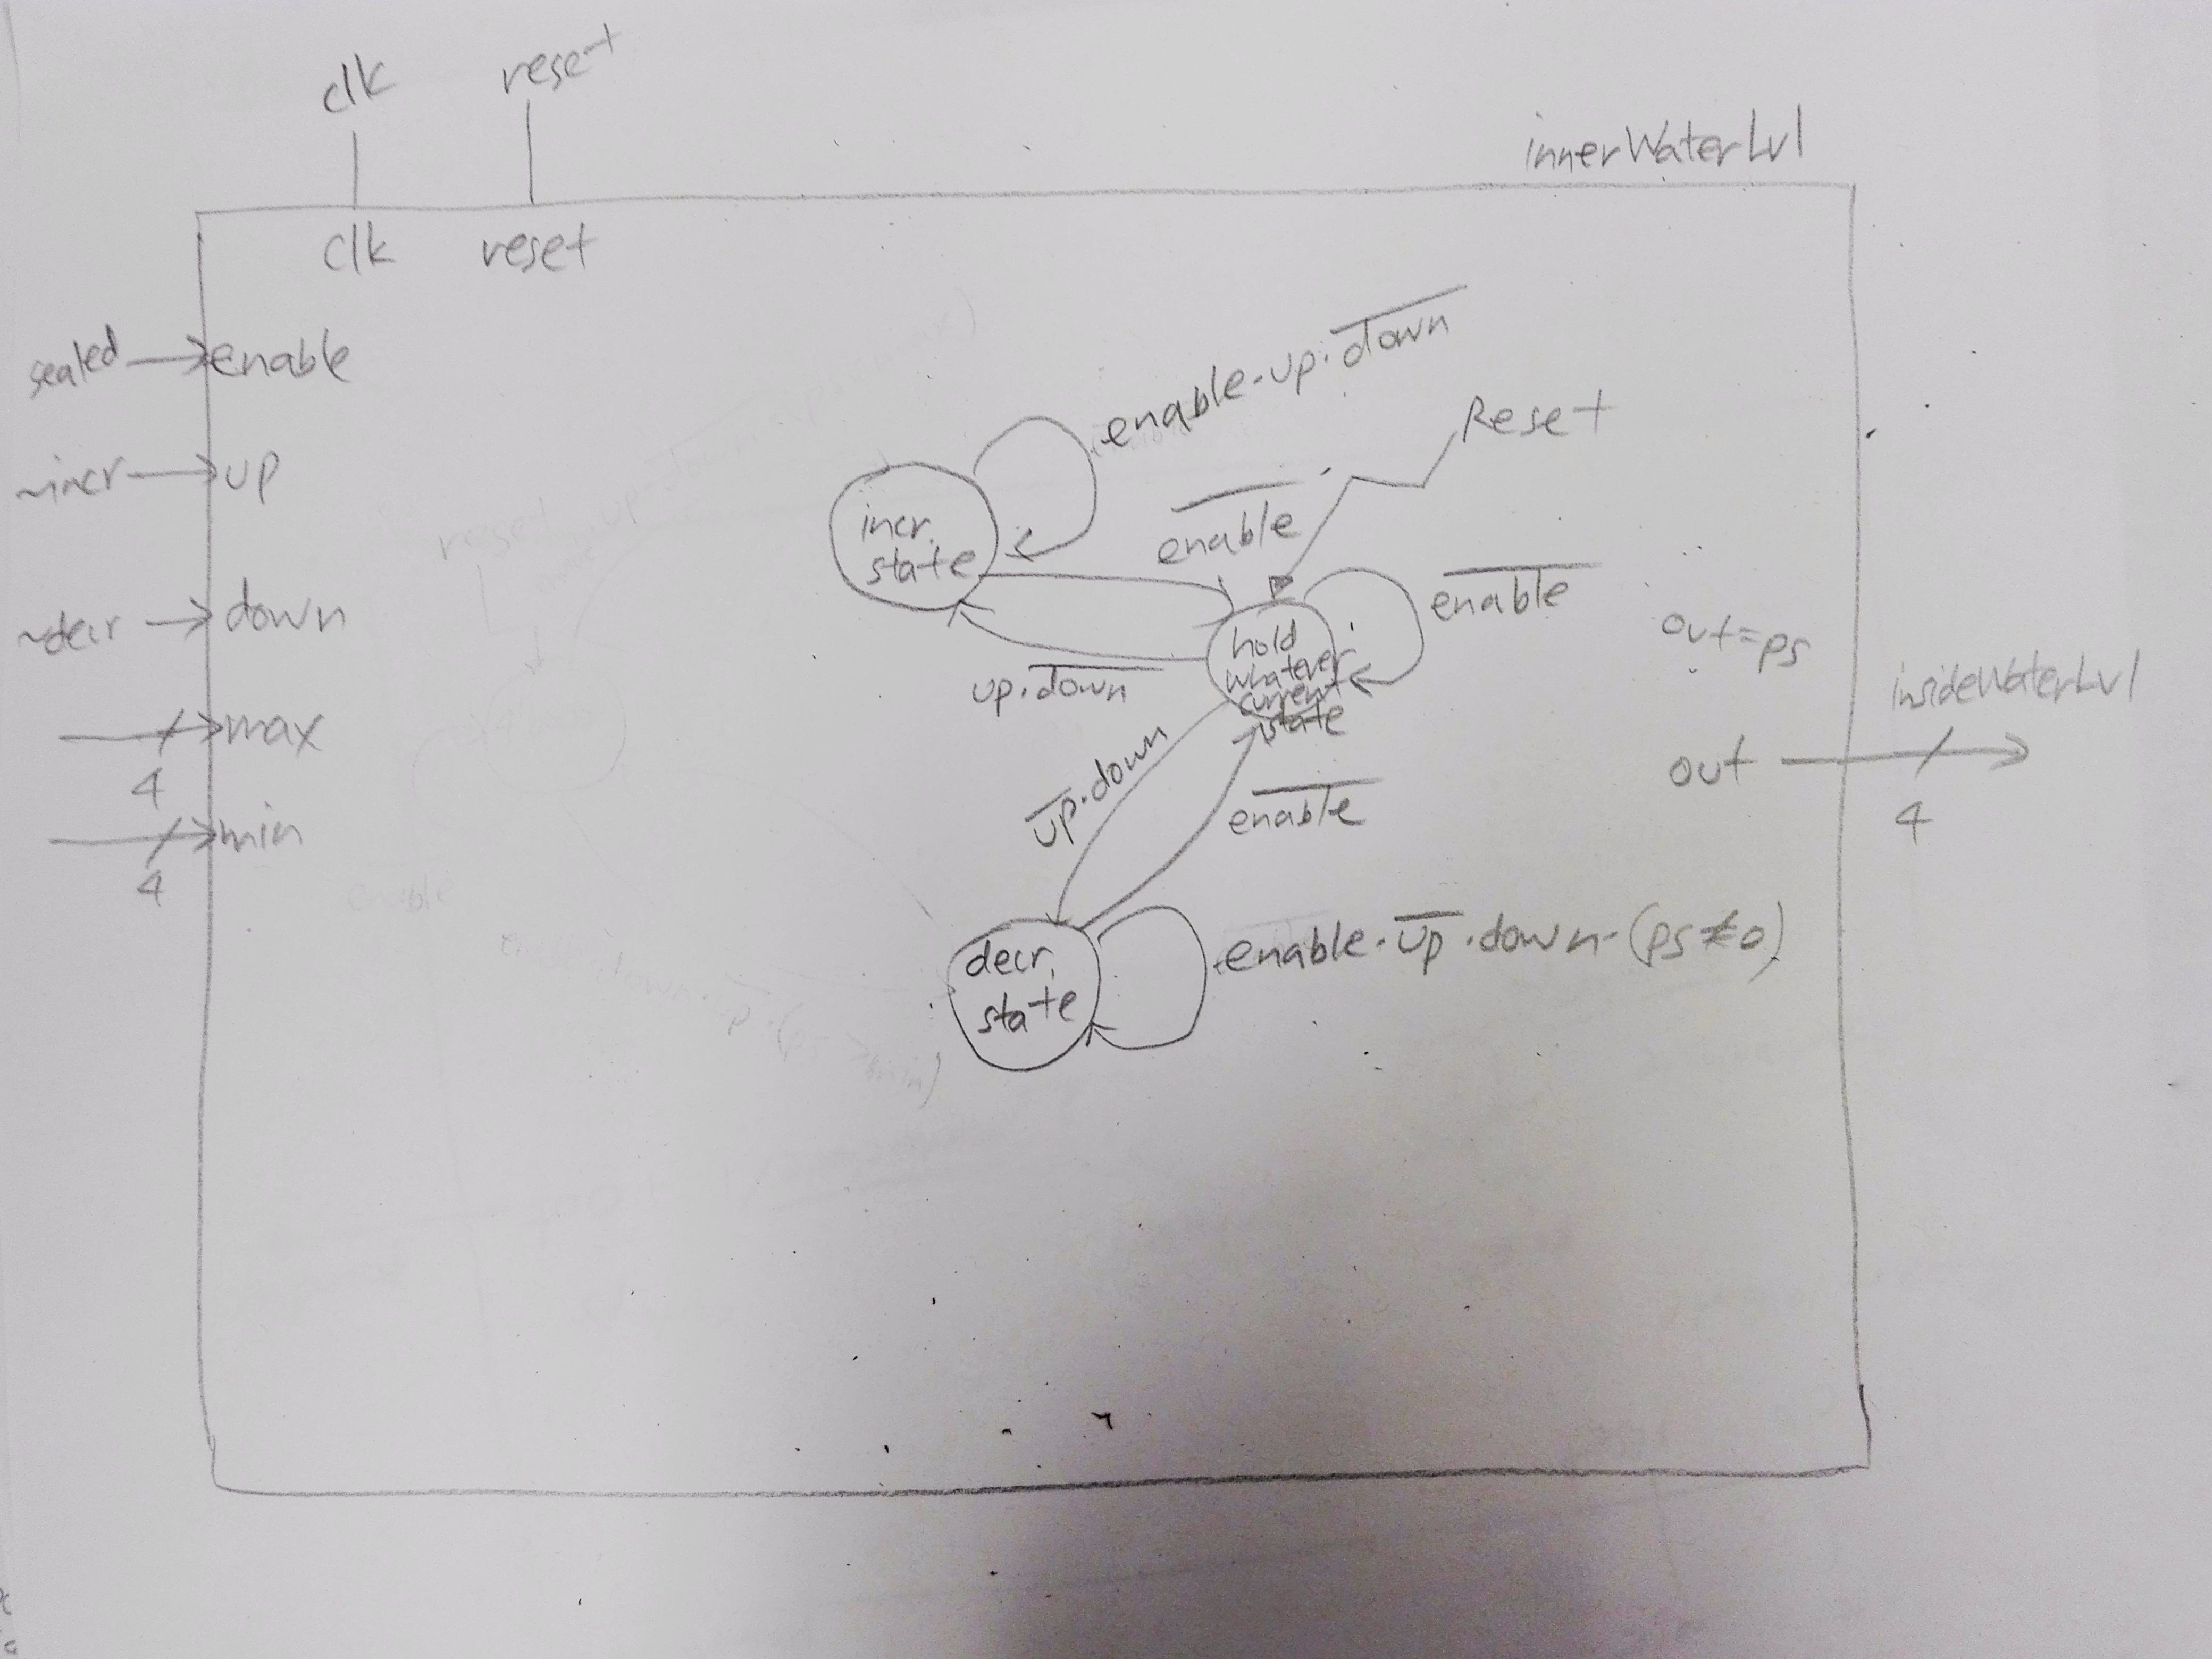
\includegraphics[width=0.6\linewidth]{figures/block_diagrams/innerWaterLvl_diagram.jpeg}
        \caption{Diagram of innerWaterLvl counter module}
        \label{fig:innerWaterLvl_diagram}
      \end{figure}

      % innerWaterLvl RTL
      \begin{figure}[H]
        \centering
        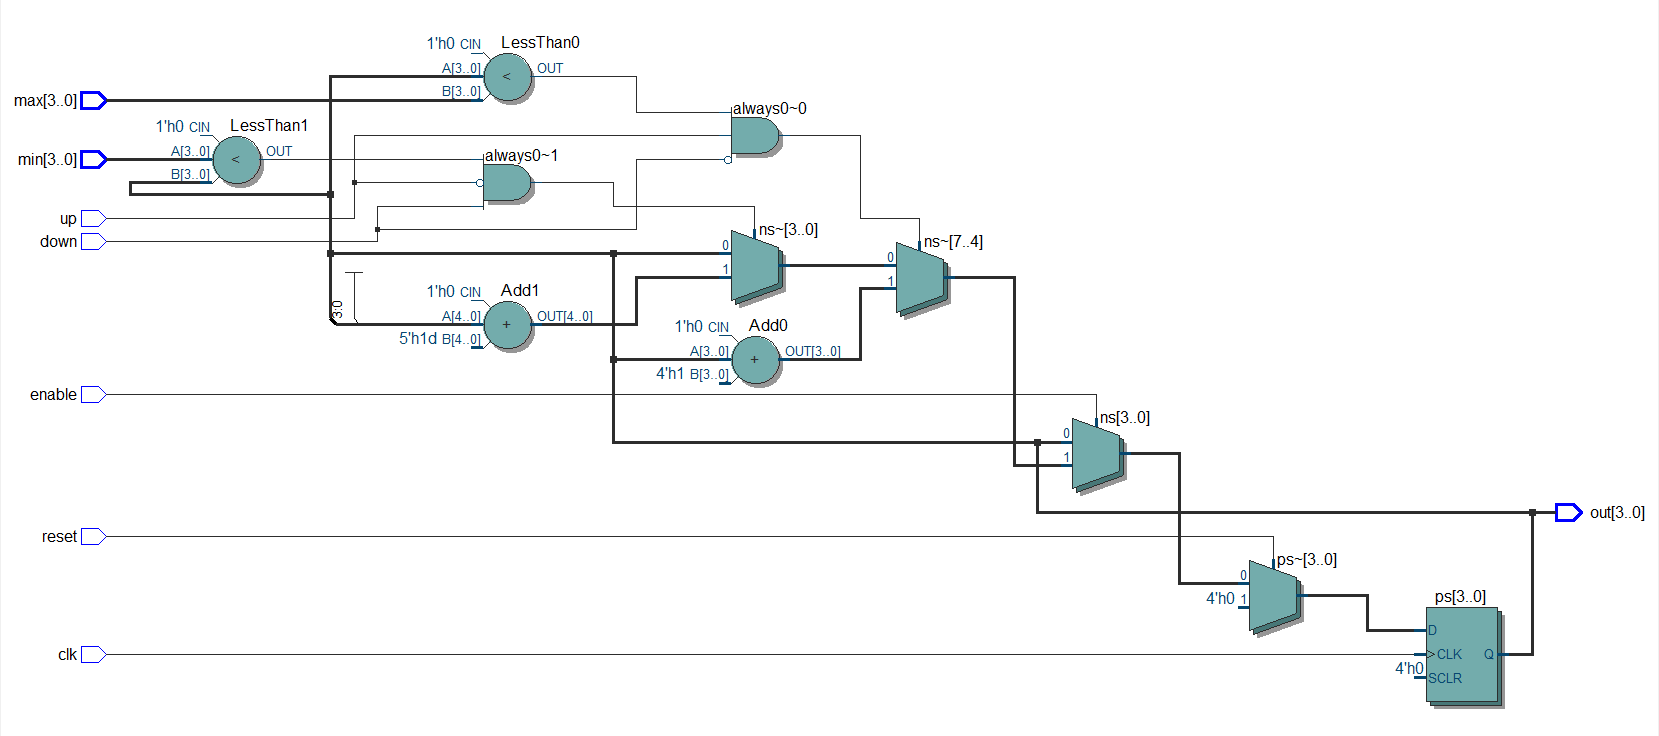
\includegraphics[width=0.75\linewidth]{figures/innerWaterlvl_RTL.PNG}
        \caption{RTL view of innerWaterLvl module}
        \label{fig:innerWaterLvl_RTL}
      \end{figure}

      \paragraph{} The gate control was implemented using combinational logic. Each gate took the relevant outside water level, the inside water level, the gateCtrl signal, and (in the case of the arrival gate) the fiveMinTillArriv and poundOccupied signal as input, and gave the state of the gate as output (1 = open/0 = closed). The logic equations are as follows:
      \begin{itemize}
        \item \lstinline{arrivGate = gateCtrl \&\& diffOkArriv \&\& ~poundOccupied \&\& fiveMinTillArriv}
        \item \lstinline{deptGate = gateCtrl \&\& diffOkDept}
      \end{itemize}

      \paragraph{} Finally, the user/environmental inputs and system outputs were connected to the input/outputs of the DE1-SoC board for visual monitoring of the signals.
      \begin{itemize}
        \item \lstinline{SW[9]} reset
        \item \lstinline{SW[8]} fiveMinTillArriv
        \item \lstinline{SW[7:4]} deptOutsideWaterLvl, \lstinline{SW[3:0]} arrivOutsideWaterLvl
        \item \lstinline{KEY[0]} decr, \lstinline{KEY[1]} incr
        \item \lstinline{KEY[2]} gateCtrl
        \item \lstinline{LED[0]} poundOccupied
        \item \lstinline{LED[4:1]} innerWaterLvl
        \item \lstinline{LED[5]} deptGate, \lstinline{LED[6]} arrivGate
      \end{itemize}


	\subsection{Test}
		\subsubsection{Test Plan}
      \paragraph{VHDL Design} Our lock system was tested under normal operating conditions. This is essentially the process of a boat passing through the lock. When the gondola arrives, the lock receives the five minutes signal. It should then seal the gates and adjust the water level to the arrivals side, then open the arrival gate. The boat enters the lock and it becomes occupied. On departure, the lock should seal the gates and adjust the water level to the departures side, then open the departure gate. The boat exits the lock and the lock becomes unoccupied.

      \paragraph{} Additionally, we tested the lock system under some unexpected failure conditions. In these cases, the lock system should fail. For example, when the lock is already occupied, another boat’s arrival signal should not open the gates; if the water levels are not close enough, the gates should not open; if the gates are not sealed, the water levels should not change; if the outside water levels (inputs to the system) are changed during operation, the system should account for it; if the system receives conflicting inputs, it should hold state to avoid faults. Finally, the reset should put the system in the expected reset state.

      \paragraph{C Program} The C Program was tested to see if the output value matched the value we computed by hand (5).

		\subsubsection{Test Specification}
      \paragraph{VHDL Design} The primary functions of the lock system were tested under various conditions: the gates, the water level adjustment, and the state of the lock (occupied/unoccupied). This was done both in simulation with iverilog and gtkwave, and on hardware with the DE1-SoC board and Signal Tap II.

      \paragraph{} The gates were tested to ensure that they open under the correct conditions. For the departure gate, it is that the difference in water levels is less than 0.3ft (1 bit binary difference, i.e. equal values). For the arrival gate, the water levels must be close enough, and it must receive the fiveMinTillArriv signal and the lock must be unoccupied in order for the gates to open. Otherwise, the gates should not open. We isolated the combinational logic for the gates into a separate module for testing purposes, and wrote a separate test bench for it.

      \paragraph{} The innerWaterLvl counter was tested to ensure that it operated within bounds. It receives input signals enable, up, down, max, and min, and outputs a 4-bit binary value (the inner water level). It should count only when enabled and given an up or down input, and only count to the max/min value (outside water levels). It should hold state when it is disabled, is given no up/down or conflicting up/down input, and it should be able to handle a changing max/min value.

      \paragraph{} The poundOccupied signal should track the state of the lock - specifically, it should only change state when the arrival gate or departure gate is opened, depending on whether there is currently a boat in the lock.

      \paragraph{C Program} Since there were no inputs to the program, it was only necessary to check that the output matched the expected value. The program outptus an integer, so we truncated our hand calculated value to an integer as well (5). We also checked to make sure the output was consistent every time we ran it.

		\subsubsection{Test Cases}
      \paragraph{VHDL Design} The lock system's three components were tested individually.

      \paragraph{} For gate control, we checked the pass case and a few fail cases.
      \begin{itemize}
        \item pass case
        \begin{itemize}
          \item inputs: fiveMinTillArriv = 1, poundOccupied = 0, diffOkArriv = 1 or diffOkDept = 1 (matching water levels)
          \item measure: whether the gate is open
          \item pass condition: the gate should open under these conditions (departure gate should open regardless of fiveMinTillArriv and poundOccupied)
        \end{itemize}

        \item fail case: water levels do not match
        \begin{itemize}
          \item inputs: diffOkArriv = 0 or diffOkDept = 0; everything else as in pass case
          \item measure: whether the gate is open
          \item pass condition: the gate should not open under these conditions
        \end{itemize}

        \item fail case: no fiveMinTillArriv signal (arrival gate only)
        \begin{itemize}
          \item input: fiveMinTillArriv = 0; everything else as in pass case
          \item measure: whether the gate is open
          \item pass condition: the gate should not open under these conditions
        \end{itemize}

        \item fail case: already occupied (arrival gate only)
        \begin{itemize}
          \item input: ponudOccupied = 1; everything else as in pass case
          \item measure: whether the gate is open
          \item pass condition: the gate should not open under these conditions
        \end{itemize}
      \end{itemize}

      \paragraph{} For the inner water level counter, we checked the effects of changing the control signals on the behaviour
      \begin{itemize}
        \item enable: the counter should not be able to count when enable = 0, regardless of other inputs
        \item up/down: when enable = 1, the counter should count up when up is pressed and down when down is pressed. When neither/both are presesd, the counter should not count.
        \item max/min: the counter should count only to the max/min value and then hold. When the max/min is changed while counting, the counter should not fault and instead count to the new value. If the counter's current state becomes out of bounds by a changing max/min, the counter should not be able to count any further out of bounds, but it should be able to count back into the bounds.
      \end{itemize}

      \paragraph{} For the poundOccupied signal, we tested change/hold state conditions.
      \begin{itemize}
        \item state change cases
        \begin{itemize}
          \item input: arrivGate = 1 \& poundOccupied = 0 or deptGate = 1 \& poundOccupied = 1
          \item measure: whether poundOccupied changes state
          \item pass condition: poundOccupied changes state
        \end{itemize}

        \item hold state case: gates do not open
        \begin{itemize}
          \item input: arrivGate = 0 \& deptGate = 0; poundOccupied = x
          \item measure: whether poundOccupied changes state
          \item pass condition: poundOccupied should not change state
        \end{itemize}

        \item hold state case: gate opens but no boat in lock (departure gate only)
        \begin{itemize}
          \item input: deptGate = 1 \& poundOccupied = 0
          \item measure: whether poundOccupied changes state
          \item pass condition: poundOccupied should not change state
        \end{itemize}
      \end{itemize}

      \paragraph{C Program} There were no inputs to the system, so the only case that needed to be tested was regular operation. In this case, the program should output the value 5, matching our hand-computed value (after integer casting truncation).


\section{Results}
  \paragraph{VHDL design} The lock system VHDL design worked as expected under normal operating parameters, and under edge cases.

  \paragraph{} When the lock receives a fiveMinTillArriv signal, the water level is adjusted, the arrival gate is opened and a boat enters, the gate is sealed and the water level adjusted again, and then the departure gate is opened and the boat exits the lock. Environmental inputs like outside water levels are input using the switches, and user inputs like the control signals for the gate and water level adjustment are through the keys. These signals behaved as expected both in simulation with iverilog/gtkwave, and visually on the outputs of the DE1-SoC board.

  \paragraph{} On reset, the lock reset to the expected reset state, namely the innerWaterLvl is set to 0 (lock drained) and the lock becomes unoccupied. Under unexpected conditions, the lock system handled the error as it should. Namely, if it was a failure condition, the property of the lock failed (gates did not open, water levels did not change). Therefore, the design successfully handled those errors.

  \paragraph{C program} The C program worked as expected. It outputs the computed value of ‘5’ every time the program is run, and since there are no inputs, there is no chance of abnormal operation.

	\subsection{Analysis of Errors}
  \paragraph{VHDL design} Ultimately, our project worked and successfully demonstrated the expected behaviour. The issues we ran into were due mostly to preliminary design faults and clock timing. At many points we found that we had failed to consider something in our original design, and this led to (at best) a minor tweak/fix, or (at worst) a major overhaul of our design and a new iteration. These problems ranged from failing to consider a variable in a logic equation to underlying misunderstandings when figuring out the required states and edge conditions in our FSMs. Another common error involved the clock edge timings for FSMs and sequential logic - sometimes we had idiosyncratic errors with a signal needing to be held for a certain number of clock cycles in order to affect the system. We solved these by checking that all our sequential logic ran on the same clock, and within the same sequential logic block. It is important to note that the modularisation of the design was very helpful in isolating the errors and minimising error propagation.

  \paragraph{C Program} Our C program also worked as expected. We had initially computed the resulting value by hand, which matched what our program's output. We ran into a few issues when trying to output the correct answer; for instance, we would try to use the address in memory in our calculations, since we had forgotten the \& for the pointer to go to the specific location in memory, but these were easily resolved.


\section{Summary \& Conclusion}
  \paragraph{Summary} This project designed a canal lock control system that allows gondolas to pass from one side to another by opening/closing gates and adjusting water levels. The lock is operated by a user, who controls it by pressing buttons to open/close the gate and increase/decrease the water level, and receives a trigger signal from the gondola to open the arrival gate. These features and behaviours were tested both in simulation with iverilog and gtkwave as well as on hardware with the DE1-SoC board. As a second component, the project involves writing a C program, using pointers rather than variables.

  \paragraph{Conclusion} Overall, this project was a good start in building simple VHDL designs. The lock system had a very simple workflow, with enough variables to make it testable for failure conditions. We were able to practice working with iverilog/gtkwave and Quartus/Signal Tap more, as well as learn about new concepts in the C language.

\section{Appendix}
	\subsection{Lock Control System}
    \subsubsection{Verilog code}
      % overall module
      \lstinputlisting[language=Verilog]{../overall.v}
      \lstinputlisting[language=Verilog]{../overall_testbench.v}

      % innerWaterLvl module
      \lstinputlisting[language=Verilog]{../innerWaterLvl.v}
      \lstinputlisting[language=Verilog]{../innerWaterLvl_testbench.v}

      % poundOccupied module
      \lstinputlisting[language=Verilog]{../poundOccupied.v}
      \lstinputlisting[language=Verilog]{../poundOccupied_testbench.v}

      % clock_divider
      \lstinputlisting[language=Verilog]{../clock_divider.v}
      \lstinputlisting[language=Verilog]{../clock_divider_testbench.v}

      % gate comb logic
      \lstinputlisting[language=Verilog]{../gate.v}
      \lstinputlisting[language=Verilog]{../gate_testbench.v}

    \subsubsection{iverilog \& gtkwave waveforms}
      % overall gtkwave
      \begin{figure} [H]
        \centering
        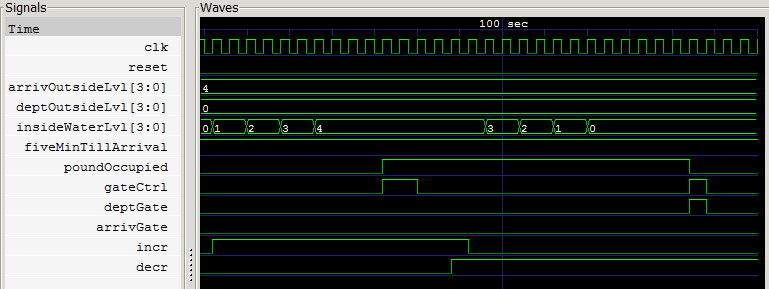
\includegraphics[width=0.75\linewidth]{figures/gtkwave/overall_gtk.png}
        \caption{waveform for overall module}
        \label{fig:overall_waveform}
      \end{figure}

      % innerWaterLvl gtkwave
      \begin{figure} [H]
        \centering
        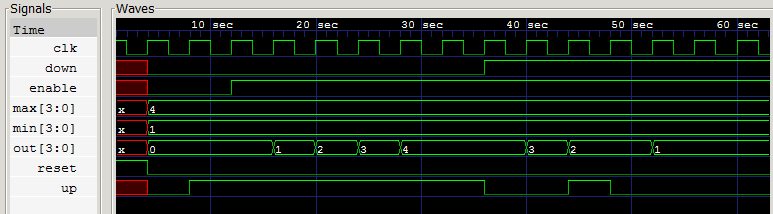
\includegraphics[width=0.75\linewidth]{figures/gtkwave/innerwatrlvl_gtk.png}
        \caption{waveform for innerWaterLvl module}
        \label{fig:innerWaterLvl_waveform}
      \end{figure}

      % poundOccupied gtkwave
      \begin{figure} [H]
        \centering
        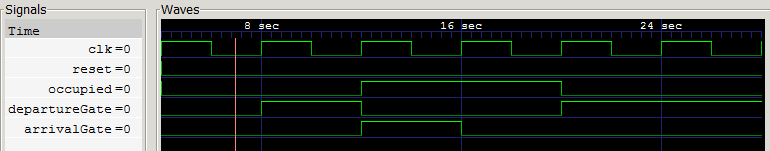
\includegraphics[width=0.75\linewidth]{figures/gtkwave/poundOccu_gtk.png}
        \caption{waveform for poundOccupied module}
        \label{fig:poundOccupied_waveform}
      \end{figure}

      % clock divider gtkwave
      \begin{figure} [H]
        \centering
        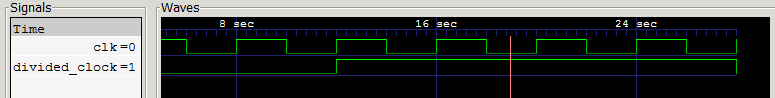
\includegraphics[width=0.75\linewidth]{figures/gtkwave/clkdiv_gtk.png}
        \caption{waveform for clock divider}
        \label{fig:clock_divider_waveform}
      \end{figure}

      % gate waveform
      \begin{figure} [H]
        \centering
        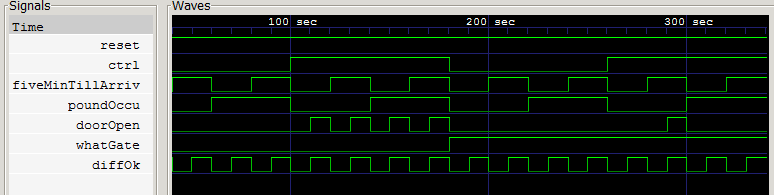
\includegraphics[width=0.75\linewidth]{figures/gtkwave/gate_gtk.png}
        \caption{waveform for gate module}
        \label{fig:gate_waveform}
      \end{figure}

      % gate truth table
      \begin{figure} [H]
        \centering
        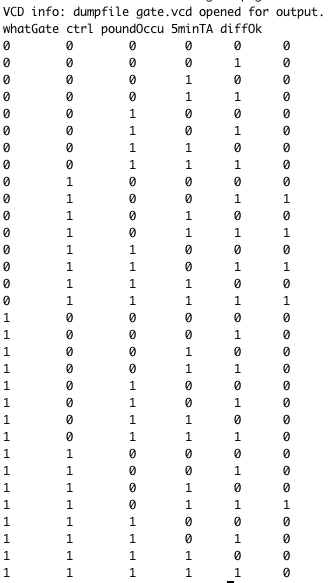
\includegraphics[width=0.55\linewidth]{figures/gate_truthtable.png}
        \caption{truth table for gate module}
        \label{fig:gate_truthtable}
      \end{figure}
    
    \subsubsection{Signal Tap II data}
      % Signal Tap data
      \begin{figure} [H]
        \centering
        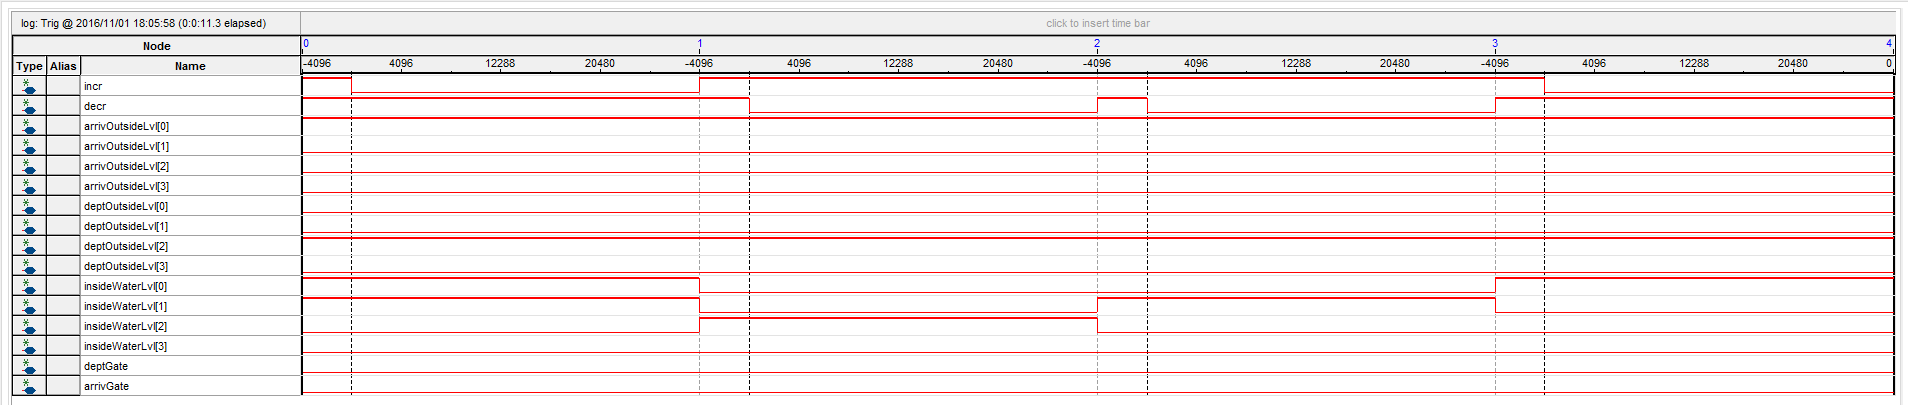
\includegraphics[width=0.75\linewidth]{figures/signaltap/stp_innerWaterLvl.PNG}
        \caption{Signal Tap data checking behaviour of the inner water level after pressing control signal}
        \label{fig:stp_innerWaterLvl}
      \end{figure}

    \subsubsection{Requirements Documentation}
      \paragraph{Abstract} At various points along the canal system of Venice, gondolas must move between areas of significantly differing water levels. In order to do so smoothly, pound locks are in place to facilitate both transportation of gondolas and maintenance of water levels. These locks are controlled by a digital system we have designed and built.

      \paragraph{Introduction} The system for controlling locks will allow gondolas to pass between areas of the canal of uneven water levels. Upon arrival, the gondola must signal the lock to initiate the process, enter the lock, wait as it is raised/lowered, and then exit the lock to continue its journey. The opening/closing of gates and raising/lowering of water levels are controlled by a lock operator.

      \paragraph{Inputs to the system}
      \paragraph{} User inputs
      \begin{itemize}
        \item fiveMinsTillArrival: signal from the gondola that it will be arriving in at least five minutes, to prompt the lock to adjust water levels and open the gates
        \item incrWaterLevel: control signal to increase the water level inside the lock, to bring the water levels inside and outside the lock close enough that the gates can open
        \item decrWaterLevel: control signal to decrease the water level inside the lock, to bring the water levels inside and outside the lock close enough that the gates can open
        \item reset: empties the lock to the lower outside water level, lets the boats out, and seals the gates
      \end{itemize}

      \paragraph{} Environmental controls
      \begin{itemize}
        \item arrivOutsideLevel: the water level outside the lock, on the arrival side, determining whether the arrival gate can open
        \item deptOutsideLevel: the water level outside the lock, on the departure side, determining whether the departure gate can open
      \end{itemize}

      \paragraph{} Internal signals
      \begin{itemize}
        \item poundOccupied: whether there is currently a gondola in the lock, since if the lock is occupied, the next boat cannot enter
        \item insideWaterLevel: the water level inside the lock, determining whether the gates can open
        \item arrivGateOpen: whether the door on the arrival side is open
        \item deptGateOpen: whether the door on the departure side is open
      \end{itemize}

      \paragraph{Outputs of major functions}
      \paragraph{} Gate control
      \begin{itemize}
        \item gateOpenClose: opens/closes the lock gates, allowing gondolas to enter/exit the lock
      \end{itemize}

      \paragraph{} Adjusting lock water level
      \begin{itemize}
        \item incrWaterLevel: increases the water level inside the lock, matching it to the outside higher water level so that the gate can open
        \item decrWaterLevel: decreases the water level inside the lock, matching it to the outside lower water level so that the gate can open
      \end{itemize}

	\subsection{C Program}
    \lstinputlisting[language=C]{../c/project2.c}

    % C program output
    \begin{figure}[H]
      \centering
      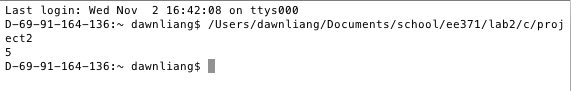
\includegraphics[width=0.75\linewidth]{figures/c/c_output.png}
      \caption{Output of C program}
      \label{fig:c_output}
    \end{figure}
\end{document}